\documentclass{scrreprt}
\usepackage{listings}
\usepackage{underscore}
\usepackage[bookmarks=true]{hyperref}
\usepackage{scrextend}
\usepackage[utf8]{inputenc}
\usepackage[english]{babel}
\usepackage{tikz}
\usepackage{xcolor}
\usepackage{graphics}
\usetikzlibrary{shapes.misc, positioning}

\usetikzlibrary{shapes.geometric, arrows}
\definecolor{orange}{HTML}{eeeeee}
\hypersetup{
    bookmarks=false,    % show bookmarks bar?
    pdftitle={Design Document},    % title
    pdfauthor={George Thomas Shanti, Prince Mathew, Riza Salahuddin},                     % author
    pdfsubject={TeX and LaTeX},                        % subject of the document
    pdfkeywords={TeX, LaTeX, graphics, images}, % list of keywords
    colorlinks=true,       % false: boxed links; true: colored links
    linkcolor=blue,       % color of internal links
    citecolor=black,       % color of links to bibliography
    filecolor=black,        % color of file links
    urlcolor=purple,        % color of external links
    linktoc=page            % only page is linked
}%

\date{}
%\title
\usepackage{hyperref}

\tikzstyle{process} = [rectangle, minimum width=4.4cm, minimum height=1cm, text centered, draw=black, fill=orange]
\tikzstyle{process1} = [rectangle, rounded corners=0.5cm, minimum width=6cm, minimum height=1.5cm, text centered, draw=black, fill=orange, align=center]
\tikzstyle{process2} = [ font=\small, rectangle, rounded corners=0.5cm, minimum width=3cm, minimum height=1.5cm, text centered, draw=black, fill=orange, align=center]
\tikzstyle{oval} = [ellipse, minimum width=3cm, minimum height=2cm, text centered, draw=black, fill=orange]
\tikzstyle{oval2} = [ellipse, minimum width=2cm, minimum height=1.5cm, text centered, draw=black, fill=orange]

\tikzstyle{func} = [rounded rectangle]
\tikzstyle{arrow} = [thick,->,>=stealth]
\tikzstyle{overlay} = [dashed, rectangle, text centered, draw=black, align=center]

\begin{document}

\begin{flushright}
    \rule{16cm}{5pt}\vskip1cm
    \begin{bfseries}
        \Huge{DESIGN DOCUMENTATION}\\
        \vspace{1.9cm}
        for\\
        \vspace{1.9cm}
        MultiFrame Hand Gesture GUI Control System using Convex Hull Algorithm\\
        \vspace{1.9cm}
        \LARGE
        Prepared by \\MDL15CS040 19 George Thomas Shanti
        \\MDL15CS082 46 Prince Mathew
        \\MDL15CS089 51 Riza Salahuddin\\
        \vspace{1.9cm}
        \today\\
    \end{bfseries}
\end{flushright}

\tableofcontents

\newpage
\chapter{Introduction}
\section{Purpose}
MultiFrame Hand Gesture GUI Control System Using Convex Hull Algorithm version 1 revision 1 - A Real time dynamic Hand Gesture Recognition GUI system to improve the interaction between user and computer. The user can use his webcam to record hand gestures which our system can use to perform Linux GUI functions in realtime.

\section{Overview}

The System Architecture provides a view into how the different blocks of the system is organized.
There are mainly four stages in this system. They are Background Subtraction, Feature Extraction,Finger-Tip Tracking, Gesture Recognition and Gesture Mapping.
The image input frames are analyzed and the hand gesture is detected from the multiple frames.
\\
\\
The Use case diagram has the different functions which are targeted at different user classes.
\\
\\
The class structure has been described in the class diagram. There is a main abstract class from which two 
sub-classes are derived; SavedGestures and DetectedGestures. \\
\\
\\
The flow of activity has been shown in the activity diagram. All the actions from the start, i.e the user gesture to the mapping and execution of the LINUX GUI function has been shown.
\\
\\
The algorithms section describe the different algorithms used in the system.
MOG2, Convex Hull, Camshift and Brute Force Matching are the main algorithms used.
  


\chapter{System Architecture}
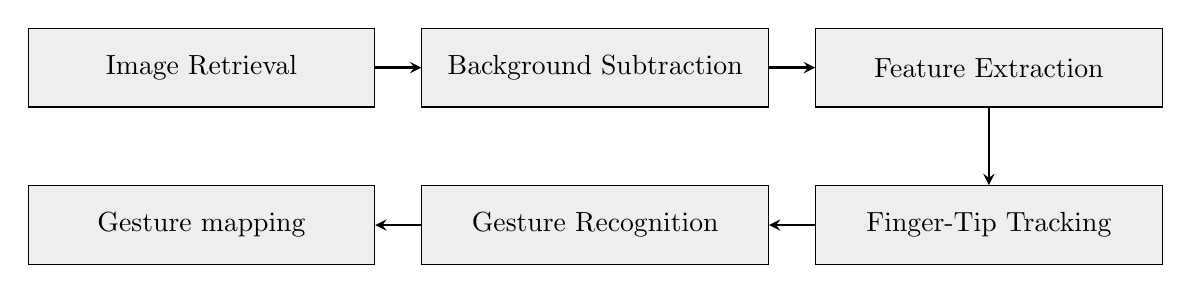
\begin{tikzpicture}[node distance=5cm]
    \node (proc1) [process] {Image Retrieval};
    \node (proc2) [process, right of = proc1] {Background Subtraction};
    \node (proc3) [process, right of = proc2] {Feature Extraction};
    \node (proc4) [process, below of = proc3, yshift = 3cm] {Finger-Tip Tracking};
    \node (proc5) [process, left of = proc4] {Gesture Recognition};
    \node (proc6) [process, left of = proc5] {Gesture mapping};
    \draw [arrow] (proc1) -- (proc2);
    \draw [arrow] (proc2) -- (proc3);
    \draw [arrow] (proc3) -- (proc4);
    \draw [arrow] (proc4) -- (proc5);
    \draw [arrow] (proc5) -- (proc6);
\end{tikzpicture}

\section{Module 1 - Image Retrieval}
The first step in this system is to retrieve the contiguous camera image frames. The user shows the hand-gesture 
and it is retrieved via the webcam. The images are captured at short intervals to accommodate multi-frame fluid hand-gestures.
\\
The camera feed is retrieved from the user's webcam using the CaptureFromCAM function provided by OpenCV.
\\
The function reads an image from the specified buffer in the memory. If the buffer is too short or contains invalid data, the empty matrix/image is returned.
\section{Module 2 - Background Subtraction}
The captured image from the camera needs to undergo background subtraction in order to recognize the gesture correctly. 
The different elements in the background has to be discarded and only the shape of the hand is retained. 
\\
The Mixture of Gaussians (MOG) method is used for foreground detection, and once the foreground is detected, we subtract the rest of the image, i. e., the background.
we need to create a background object using the function, cv.createBackgroundSubtractorMOG(). 
It has some optional parameters like length of history, number of gaussian mixtures, threshold etc. 
Then we use backgroundsubtractor.apply() method to get the foreground mask.
\section{Module 3 - Feature Extraction}
The next step is to find the fingertip locations in the recorded image from the background subtracted image.
To recognize the fingertips we use the Convex Hull algorithm. 
\\
The locations of the fingertips on the screen are detected by finding the Convex hull of the 
hand and marking the peaks. This process is done in realtime and the extracted location changes
 with every frame. 
 
 The function find the convex hull of a 2D point set using the Sklansky’s algorithm
 that has O(N logN) complexity in the current implementation. The algorithm consisted of two parts. 
 Part 1 was intended to take a simple polygon and return a maximal polygon (monotonic in both the 
 horizontal and vertical directions). Part 2 was Sklansky's original algorithm, which
 was guaranteed to work on the output of part 1, since maximal polygons are weakly externally visible,
 and it is proven that Sklansky's original algorithm works for such polygons.

\section{Module 4 - Finger-Tip Tracking}
After extracting the finger tip information, we need to track the finger tips over multiple frames. 
cv.camShift() is the function that is used. 
Continuously Adaptive Mean Shift Algorithm (CAMShift) is used to detect the changes from frame to frame. 
The probability distribution of the first frame is taken as a reference for the second frame, 
the probability distribution of the second frame is taken for the third frame and so on and so forth.

\section{Module 5 - Gesture Recognition}
The convex hull and convexity defects along with the results of the CAMShift algorithm are 
used to create a mathematical state of the currently recorded gesture. This state is compared 
with the states of the saved gestures and the closest candidate is chosen.

We use Brute Force matching to find the closest saved gesture. First we create 
ORB descriptors (Oriented FAST (Features from accelerated segment test) and Rotated BRIEF 
(Binary Robust Independent Elementary Features)) and these descriptors are checked by using the 
Brute Force matcher.  

\section{Module 6 - Gesture Mapping}

Once the correct gesture has been identified, 
the corresponding class object is accessed to procure the GUI function that has been saved 
for that particular gesture. The function is first executed, and then the daemon starts listening 
for the next gesture.

\chapter{Data Description}

\section{Data Flow Diagram}

\subsection{Level 0}
\resizebox{\columnwidth}{!}{
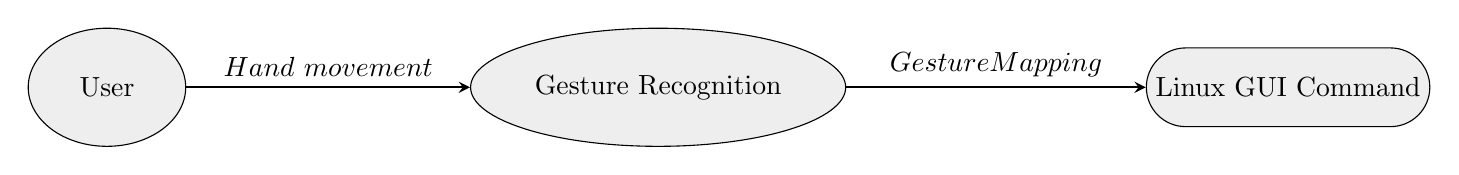
\begin{tikzpicture}[node distance=7cm]
    \node (proc1) [oval2]{User};
    \node (proc2) [oval2, minimum width=10mm,right of = proc1]{Gesture Recognition};
    \node (proc3) [process1,minimum size=10 mm, right of = proc2,xshift= 10 mm]{Linux GUI Command};

    \draw[arrow] (proc1)--(proc2) node[midway,above,rotate=0] {$Hand\ movement$};
    \draw[arrow] (proc2)--(proc3) node[midway,above,rotate=0] {$Gesture Mapping$};
%    \draw [black] ([yshift=0.2cm]proc3.west)--([yshift=0.2cm]proc3.east);

\end{tikzpicture}}
\\
\subsection{Level 1}
\resizebox{\columnwidth}{!}{
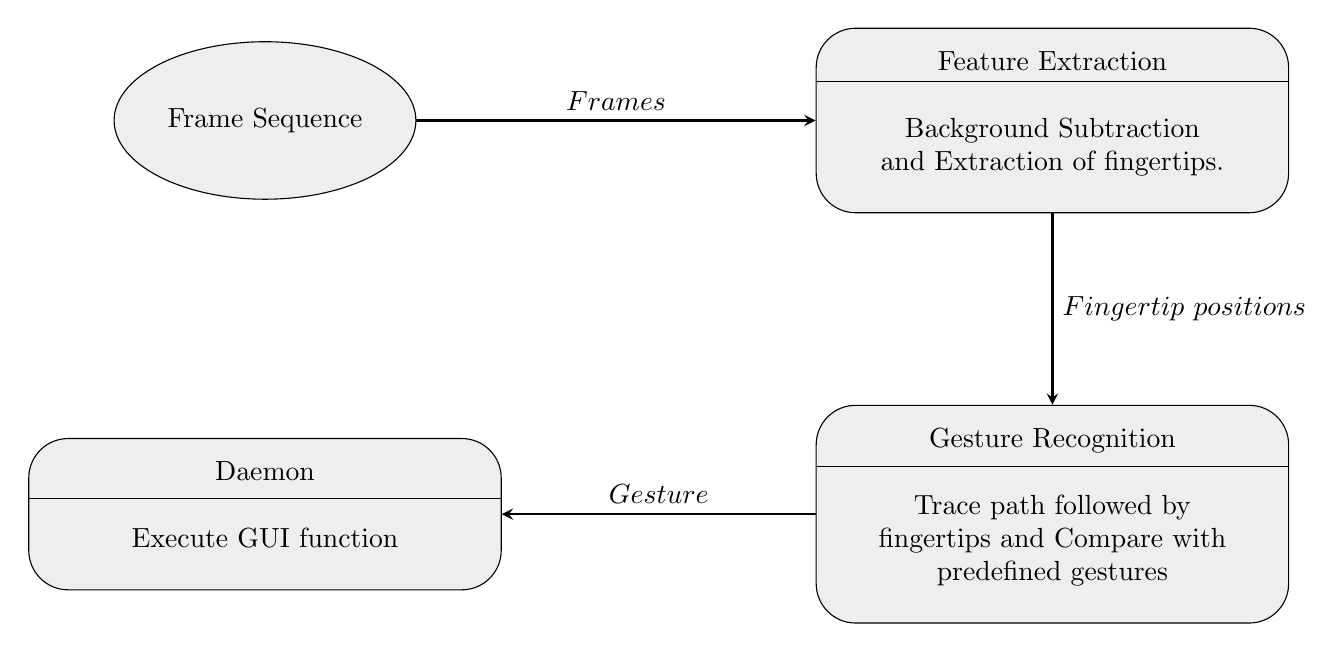
\begin{tikzpicture}[node distance=2cm]
    \node (proc1) [oval]{Frame Sequence};
    \node (proc2) [process1, right of = proc1, xshift=8 cm]{\\Feature Extraction\\\\
    Background Subtraction\\
    and Extraction of fingertips.\\};
    \node (proc3) [process1, below of = proc2, yshift=-3cm]{\\Gesture Recognition\\\\
    Trace path followed by\\
    fingertips and Compare with\\
    predefined gestures\\};
    \node (proc4) [process1, left of = proc3, xshift=-8cm]{\\Daemon\\\\Execute GUI function\\};
    \draw[arrow] (proc1)--(proc2) node[midway,above,rotate=0] {$Frames$};
    \draw[arrow] (proc2)--(proc3) node[midway,right,rotate=0]{$Fingertip\ positions$};
    \draw[arrow] (proc3)--(proc4) node[midway,above,rotate=0] {$Gesture$};
    \draw [black] ([yshift=0.5cm]proc2.west)--([yshift=0.5cm]proc2.east);
    \draw [black] ([yshift=0.6cm]proc3.west)--([yshift=0.6cm]proc3.east);
    \draw [black] ([yshift=0.2cm]proc4.west)--([yshift=0.2cm]proc4.east);
\end{tikzpicture}}

\subsection{Level 2}
\resizebox{\columnwidth}{!}{
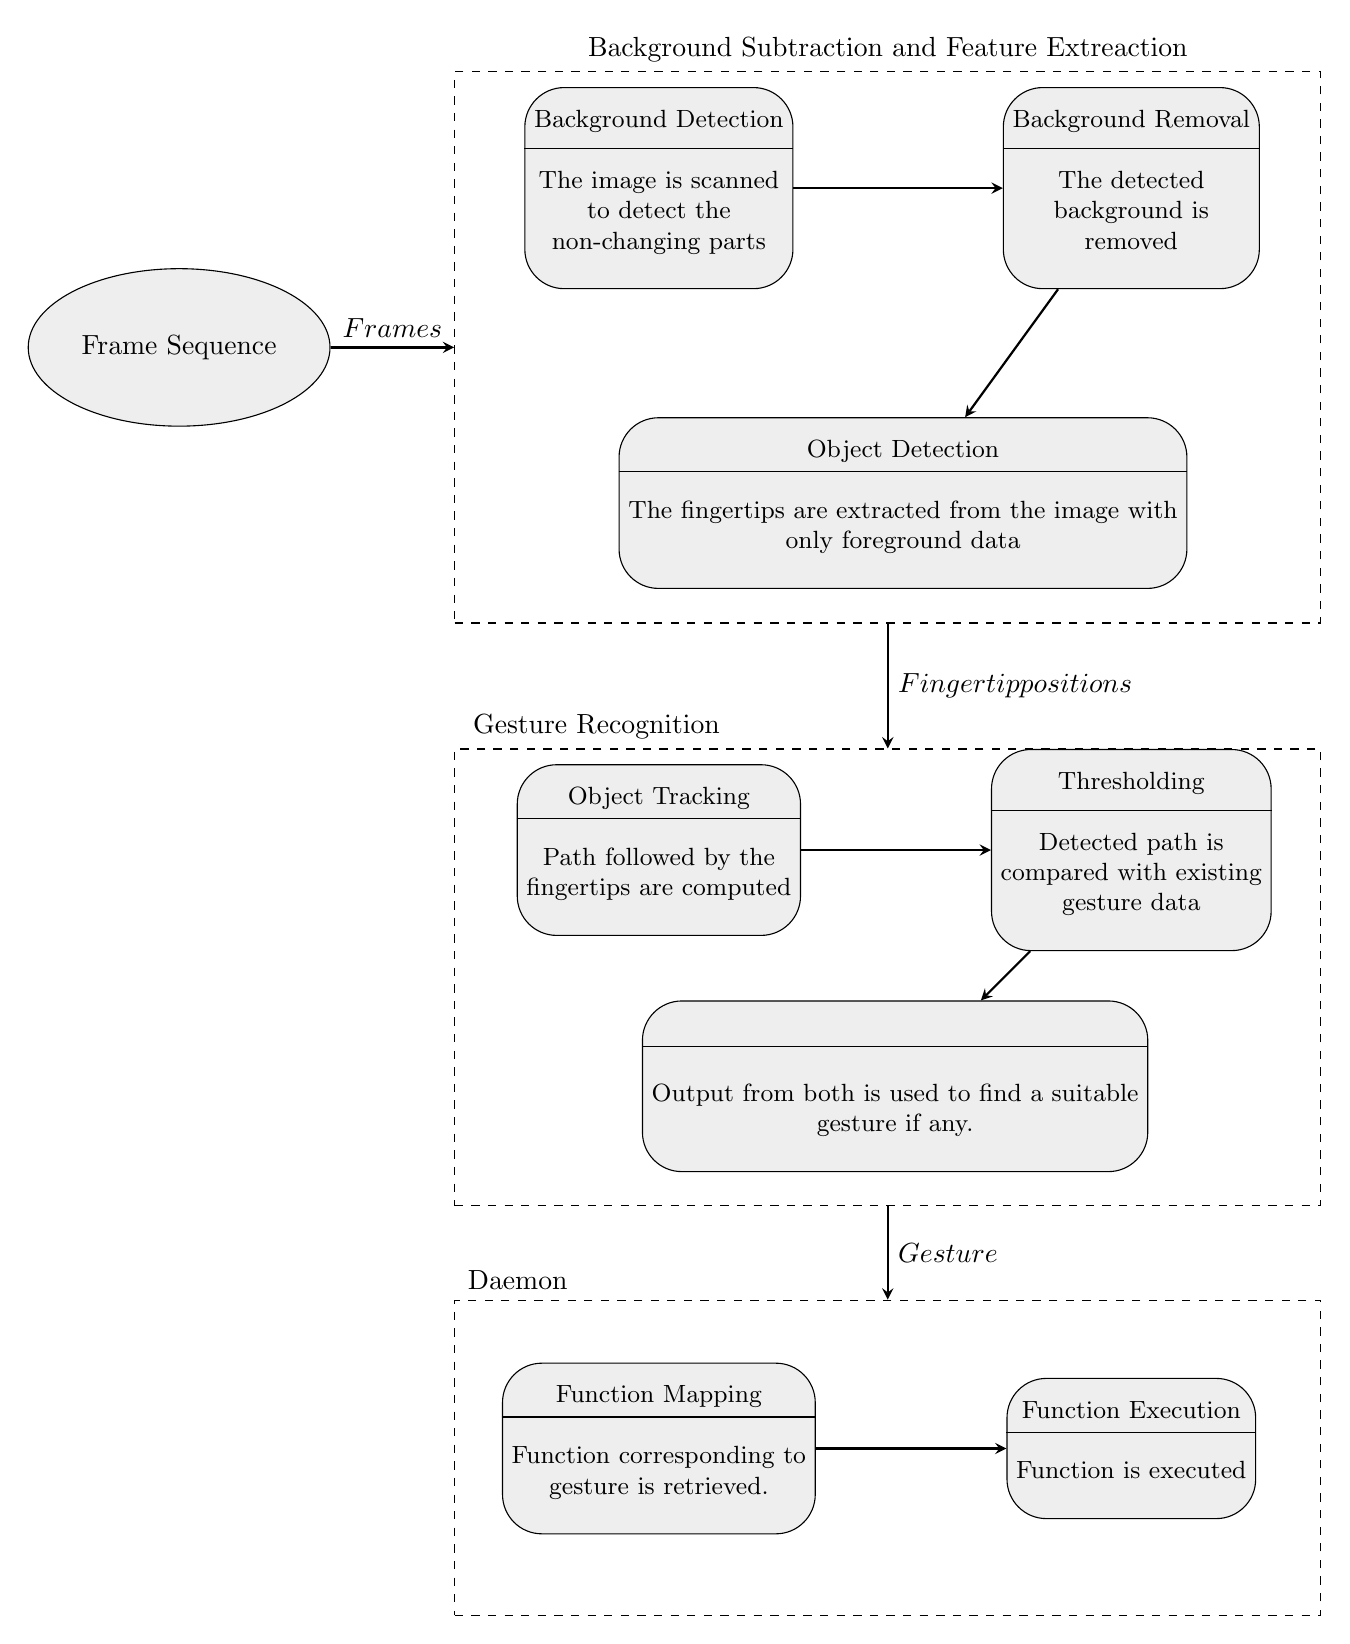
\begin{tikzpicture}[node distance=0cm]
    \node (proc1) [oval]{Frame Sequence};

    \node (over1) [overlay, label=above:Background Subtraction and Feature Extreaction, minimum width = 11cm, minimum height = 7cm, right of = proc1, xshift=9cm]{};

    \node (proc2) [process2, below=of over1.north west, xshift=2.6cm, yshift=-0.2cm]{\\Background Detection\\\\
    The image is scanned\\
    to detect the\\
    non-changing parts\\};


    \node (proc3) [process2, right of = proc2, xshift=6cm]{\\Background Removal\\\\
    The detected\\
    background is\\
    removed\\};

    \node (proc4) [process2, left of = proc3, xshift=-2.9cm, yshift=-4cm]{\\Object Detection\\\\
    The fingertips are extracted from the image with\\
    only foreground data\\};

    \draw [arrow] (proc1)--(over1) node[midway,above,rotate=0] {$Frames$};
    \draw [black] ([yshift=0.5cm]proc2.west)--([yshift=0.5cm]proc2.east);
    \draw [black] ([yshift=0.5cm]proc3.west)--([yshift=0.5cm]proc3.east);
    \draw [black] ([yshift=0.4cm]proc4.west)--([yshift=0.4cm]proc4.east);
    \draw [arrow] (proc2)--(proc3) node[midway, above]{$$};
    \draw [arrow] (proc3)--(proc4) node[midway, above]{$$};
    \node (over2) [overlay, label={[xshift=-3.7cm]Gesture Recognition}, minimum width = 11cm, minimum height = 5.8cm, right of = over1, yshift=-8cm]{};

    \node (proc5) [process2, below=of over2.north west, xshift=2.6cm, yshift=-0.2cm]{\\Object Tracking\\\\
    Path followed by the\\
    fingertips are computed\\};

    \node (proc6) [process2, right of = proc5, xshift=6cm]{\\Thresholding\\\\
    Detected path is\\
    compared with existing\\
    gesture data\\};

    \node (proc7) [process2, left of = proc6, xshift=-3cm, yshift=-3cm]{\\\\\\
    Output from both is used to find a suitable\\
    gesture if any.\\};
    \draw [arrow] (over1)--(over2) node[midway, right]{$Fingertip positions$};
    \draw [black] ([yshift=0.4cm]proc5.west)--([yshift=0.4cm]proc5.east);
    \draw [black] ([yshift=0.5cm]proc6.west)--([yshift=0.5cm]proc6.east);
    \draw [black] ([yshift=0.5cm]proc7.west)--([yshift=0.5cm]proc7.east);
    \draw [arrow] (proc5)--(proc6) node[midway, below]{$$};
    \draw [arrow] (proc6)--(proc7) node[midway, below]{$$};

    \node (over3) [overlay, label={[xshift=-4.7cm]Daemon}, minimum width = 11cm, minimum height = 4cm, right of = over2, yshift=-6.1cm]{};

    \node (proc8) [process2, below=of over3.north west, xshift=2.6cm, yshift=-0.8cm]{\\Function Mapping\\\\
    Function corresponding to\\
    gesture is retrieved.\\};

    \node (proc9) [process2, right of = proc8, xshift=6cm]{\\Function Execution\\\\
    Function is executed\\};
    \draw [arrow] (proc8)--(proc9) node[midway, below]{$$};

    \draw [arrow] (over2)--(over3) node[midway, right]{$Gesture$};

    \draw [black] ([yshift=0.4cm]proc8.west)--([yshift=0.4cm]proc8.east);
    \draw [black] ([yshift=0.2cm]proc9.west)--([yshift=0.2cm]proc9.east);

\end{tikzpicture}}

\section{Use case diagram}
\begin{center}
    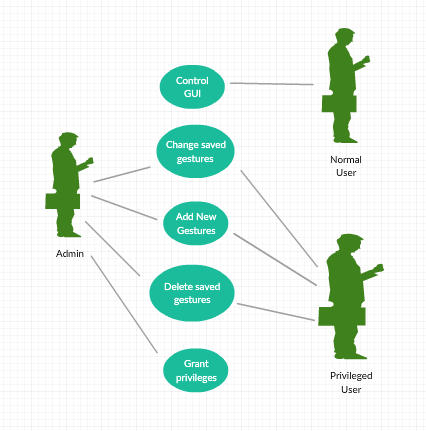
\includegraphics{usecase.png}
\end{center}
\section{Class diagram}
\begin{center}
    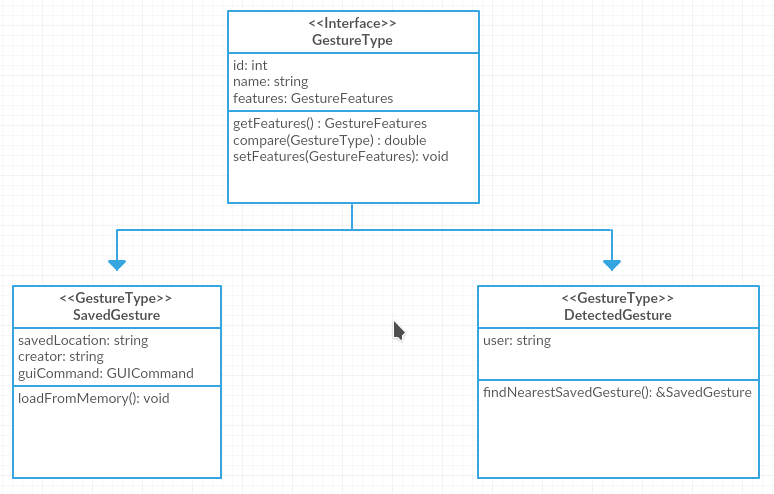
\includegraphics[width=14cm]{classdiagram.png}
    \vspace{10cm}
    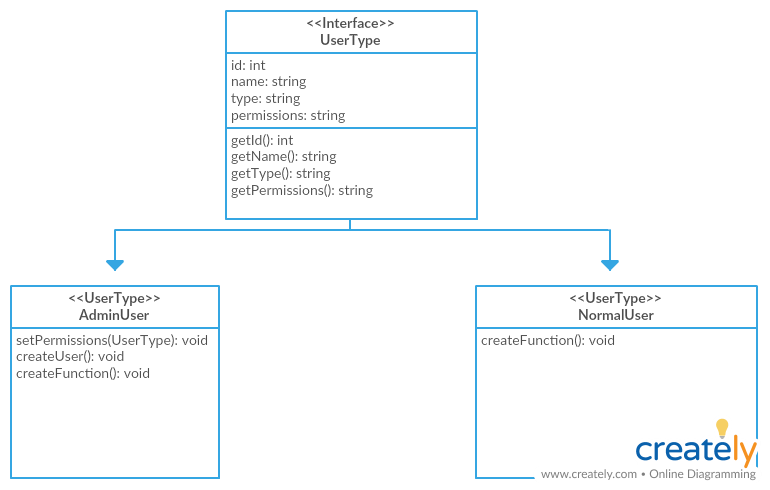
\includegraphics[width=14cm]{UserClass.png}
\end{center}
\section{Activity diagram}
\begin{center}
    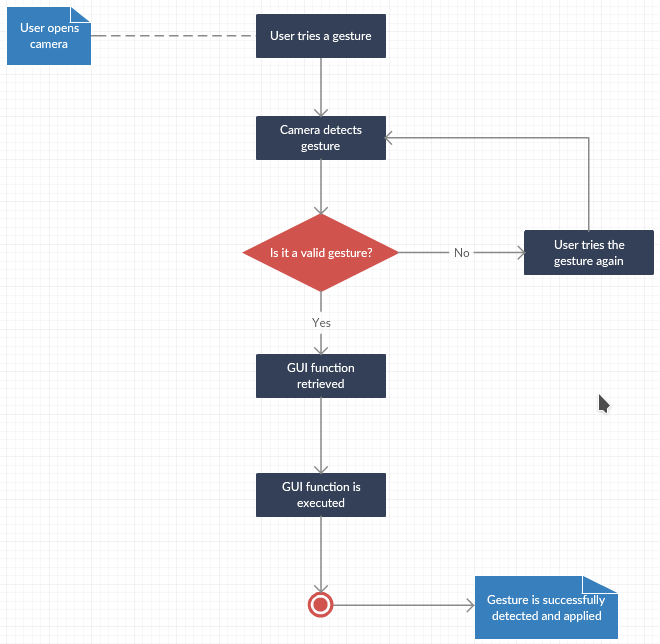
\includegraphics[scale=0.8]{activitydiagram.png}
\end{center}

\chapter{Algorithms}
Explain the pseudocodes of the algorithms that will be used in the implementation of the project.
\section{Overall algorithm}
\begin{itemize}
    \item Input: A set of contiguous image frames
    \item Output: The mapped GUI function
    \item Method:
    \begin{enumerate}
        \item Calculate the foreground using MOG2 background subtraction algorithm.
        \item Detect the fingertips using the Convex Hull algorithm.
        \item Track the finger gesture using Continuously Adaptive Mean Shift (CAMshift) algorithm.
        \item Save the above tracked graph to a DetectedGesture object.
        \item Find the closest SavedGesture object and execute the GUI function.
    \end{enumerate}
\end{itemize}
\section{Background subtraction}
\begin{enumerate}
    \item Purpose: To find the Region of Interest by subtracting the background from the image frame.
    \item Input: Image frames with foreground and background.
    \item Output: Image frames with only foreground. 
    \item Method:
    \begin{itemize}
        \item Model each background pixel by a mixture of K Gaussian distributions (K = 3 to 5)
        \item Calculate the weights of the mixture which represent the time proportions that those colours stay in the scene.
        \item Remove the colours are which stay longer and more static.
    \end{itemize}
\end{enumerate}
\section{Convex Hull}
\begin{itemize}
    \item Purpose: To find the positions of the fingertips in the image frame.
    \item Input: Image frames with background subtracted.
    \item Output: List of Convex Hull peaks
    \item Method:
    \begin{enumerate}
        \item Threshold the image, and retrieve the points in the plane. Let's say there are P points.
        \item Initialize p as leftmost point.
        \item Do following while we don’t come back to the first (or leftmost) point.
        \begin{enumerate}
            \item The next point q is the point such that the triplet (p, q, r) is counterclockwise for any other point r.
            \item next[p] = q (Store q as next of p in the output convex hull).
            \item p = q (Set p as q for next iteration).
        \end{enumerate}
    \end{enumerate}
\end{itemize}
\section{CAMShift}
\begin{itemize}
    \item Purpose: To map the positions of the fingertips in the multiple frames to one fluid motion, in the form of lines/curves in a 2D plane.
    \item Input: Sequence of frames with Convex Hull peaks.
    \item Output: 2D plane with a set of lines/curves representing the fluid motion of the fingertips.
    \item Method:
    \begin{enumerate}
        \item Set the calculation region of the probability distribution equal to the whole frame.
        \item Choose the initial location of the two-dimensional mean shift search window.
        \item Calculate the colour probability distribution in the 2D region centred on the search window location in an area slightly larger than the mean shift window size.
        \item Perform the search of the maximum density probability using the mean shift parameter for convergence or for setting the number of iterations. Store the zero moment (area or size) and middle position.
        \item For the next image frame, place the search window in the middle position fixed in step 4, and set the window size in conformity to the last moment. Go to step 3. 
    \end{enumerate}
\end{itemize}
\section{Brute Force Matching}
\begin{itemize}
    \item Purpose: To match the DetectedGesture to a SavedGesture, and execute the corresponding GUI function.
    \item Input: The feature objects encoded in the SavedFeature and DetectedFeature objects.
    \item Output: A quantity representing the closeness of the two gestures.
    \item Method:
    \begin{enumerate}
        \item For a given keypoint K1 from the first set, take every keypoint in the second set and calculate the distance.
        \item Distance formula used is Euclidean distance. The sum of the distances on each dimension is finally used to calculate the returned quantity.
        \item cv2.NORM2 can be used to find the BFMatch value between two sets (of points)
        \item The Euclidean Distance sum is normalized and returned.
    \end{enumerate}
\end{itemize}

\chapter{Conclusion}
MultiFrame Hand Gesture GUI Control System using Convex Hull Algorithm is a suitable system to perform basic GUI functions using dynamic hand gestures. 
\\

The input feed is divided into individual frames taken at multiple intervals. These image frames are then passed into the Background Subtraction Module which isolates the Region of Interest.
The images are then quantized to grayscale, and passed through the Convex Hull Algorithm to extract the fingertip points.
Then, the motion of the fingertips is tracked using the tracking algorithm from the multiple frames, and the dynamic gesture is retrieved and saved as the detected gesture.
This object is then compared using Brute Force Matching against all the saved gestures to find a suitable match. Once a match is found, the corresponding GUI function is executed.
\\

The algorithms specified in Section 4 are optimized and relatively fast, and are highly accurate.
\\

Hence, this is an easy-to-use and a highly expandable system for interfacing with the personal computer.
\begin{thebibliography}{999}
\addcontentsline{toc}{chapter}{References}

\bibitem{ } REAL TIME HAND GESTURE RECOGNITION
SYSTEM FOR DYNAMIC APPLICATIONS , Siddharth S. Rautaray , Anupam Agrawal, 2012

\bibitem{ } Natural Human- Machine Interface using an Interactive Virtual Blackboard
Conic N., Cerseato P., De \& Natale, F. G. B. (2007)
 
\bibitem{ } A Real Time Vision-Based Hand Gesture Interaction
Pang, Y. Y., Ismail, N. A., \& Gilbert, P. L. S., (2010)

\bibitem{ } A Fuzzy Brute Force Matching Method for Binary Image Features 
Erkan Bostanci, Nadia Kanwal, Betul Bostanci \& Mehmet Serdar Guzel

\bibitem{ } Object Tracking Using CamShift Algorithm and Multiple Quantized Feature Spaces 
ohn G. Allen, Richard Y. D. Xu \& Jesse S. Jin 

\end{thebibliography}

\end{document}
